\documentclass{article}

\usepackage{polski}
\usepackage[utf8]{inputenc}
\usepackage{indentfirst}
\usepackage{color}
\usepackage{graphicx}

\newcommand{\TODO}[1]{\textcolor{blue}{TODO: #1}}
\newcommand{\ang}[1]{ang.~{\itshape #1}}

\begin{document}

\title{Metody odkrywania wiedzy \\%
{\large Klasyfikacja -- dokumentacja końcowa} }

\author{Jakub Cichanowicz \and Artur Sawicki}

\maketitle

\section{Analiza i przygotowanie danych}
Zbiór danych składa się z 12 atrybutów. Część z nich ma braki, które należy uzupełnić, gdyż nie wszystkie algorytmy radzą sobie z brakami danych.

\subsection{Klasa pasażerska}

Atrybut ten nie ma braków danych. Rozkład przedstawia się następująco:
\begin{center}
    \begin{tabular}{| l | l | l |}
    \hline
	1   & 2  & 3 \\ \hline
    216 & 184 & 491 \\
    \hline
    \end{tabular}
\end{center}

Z poniższego wykresu można wywnioskować, że atrybut ten miał wpływ na przeżycie.\\
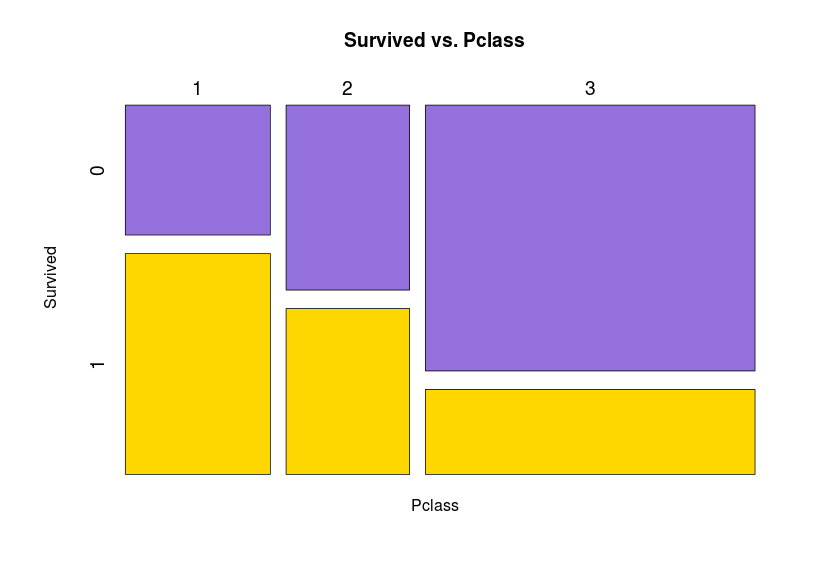
\includegraphics[scale=0.4]{images/survived-vs-pclass.png}

\subsection{Płeć}

Atrybut ten również nie ma braków, a rozkład przedstawia się następująco.
\begin{center}
    \begin{tabular}{| l | l |}
    \hline
	female &  male \\ \hline
	314  &  577 \\
    \hline
    \end{tabular}
\end{center}

Poniższy wykres pokazuje, że płeć ma wpływ na przeżycie.
\begin{center}
	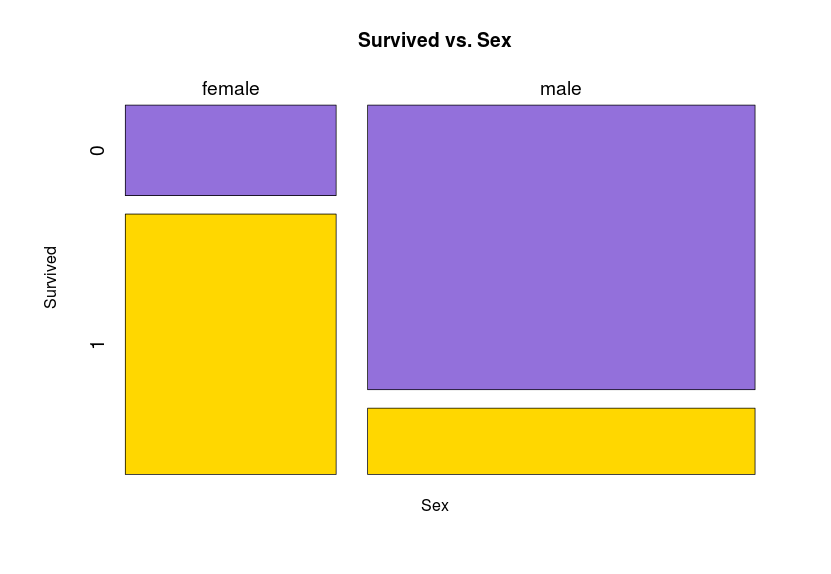
\includegraphics[scale=0.40]{images/survived-vs-sex.png}
\end{center}

\subsection{Wiek}

Wiek jest atrybutem numerycznym o rozkładzie:
\begin{center}
    \begin{tabular}{| l | l | l | l | l | l | l |}
    \hline
Min. & 1st Qu. & Median   & Mean & 3rd Qu.  &  Max.  &  NA's  \\ \hline
0.42  & 20.12  & 28.00  & 29.70 &  38.00  & 80.00   &  177 \\
    \hline
    \end{tabular}
\end{center}

Wykres przedstawiony poniżej pokazuje, że wiek nie wpływa w oczywisty sposób na przeżywalność.

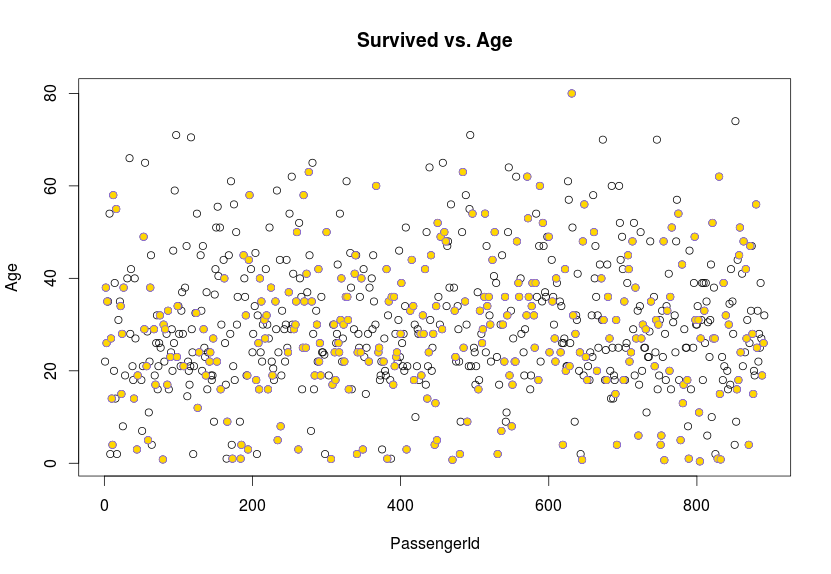
\includegraphics[scale=0.40]{images/survived-vs-age.png}

Żółtymi kropkami oznaczone są osoby, które przeżyły, natomiast białymi te, które nie przeżyły. Braki danych zastąpione zostały w eksperymentach medianą dla płci.

\subsection{Liczba rodzeństwa/małżonków na pokładzie}

Nie ma braków danych. Rozkład przedstawia się następująco:
\begin{center}
    \begin{tabular}{| l | l | l | l | l | l | l |}
    \hline
0 &  1  & 2  & 3  & 4 &  5 &  8  \\ \hline
608 & 209 & 28 & 16 & 18 &  5 &  7 \\
    \hline
    \end{tabular}
\end{center}

Wykres pokazuje, że wpływ atrybutu nie jest jednoznaczny.

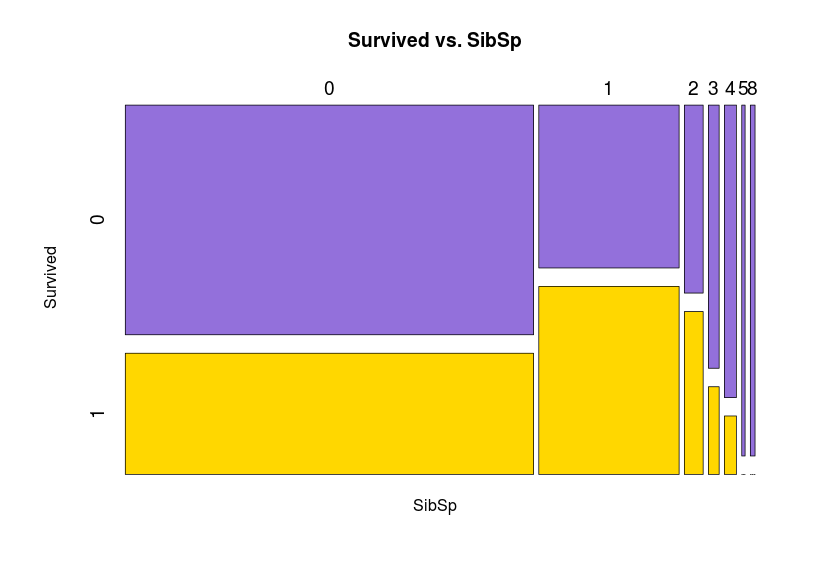
\includegraphics[scale=0.40]{images/survived-vs-sibsp.png}

\subsection{Liczba dzieci/rodziców na pokładzie}

Nie ma braków danych. Rozkład przedstawia się następująco:
\begin{center}
    \begin{tabular}{| l | l | l | l | l | l | l |}
    \hline
 0  & 1  & 2 &  3  & 4 &  5  & 6 \\ \hline
 678 & 118 & 80 &  5  & 4  & 5 &  1 \\
    \hline
    \end{tabular}
\end{center}

Wykres pokazuje, że wpływ atrybutu nie jest jednoznaczny.
\begin{center}
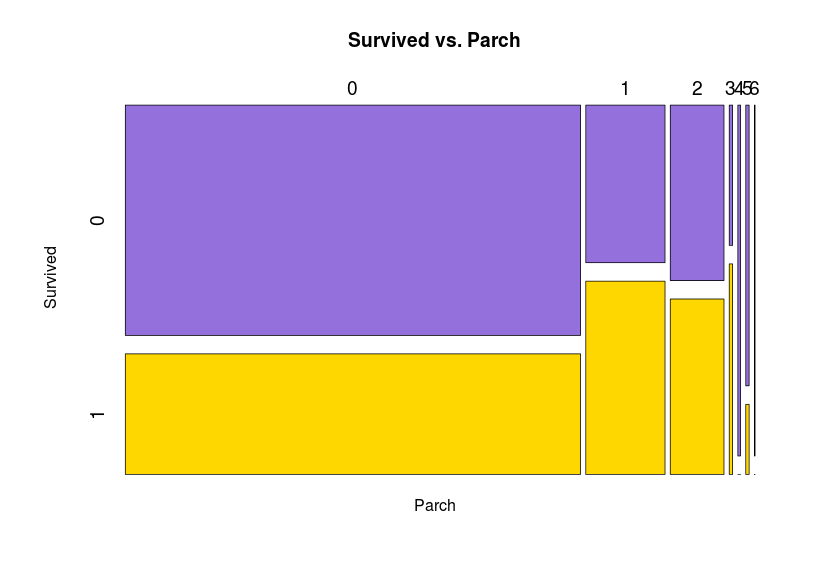
\includegraphics[scale=0.40]{images/survived-vs-parch.png}
\end{center}

\subsection{Opłata za bilet}

Na wykresie widać, że wpływ atrybutu nie jest jednoznaczny, ale większość osób, które kupiły drogie bilety przeżyli (żółte kropki to osoby, które przeżyły).
\begin{center}
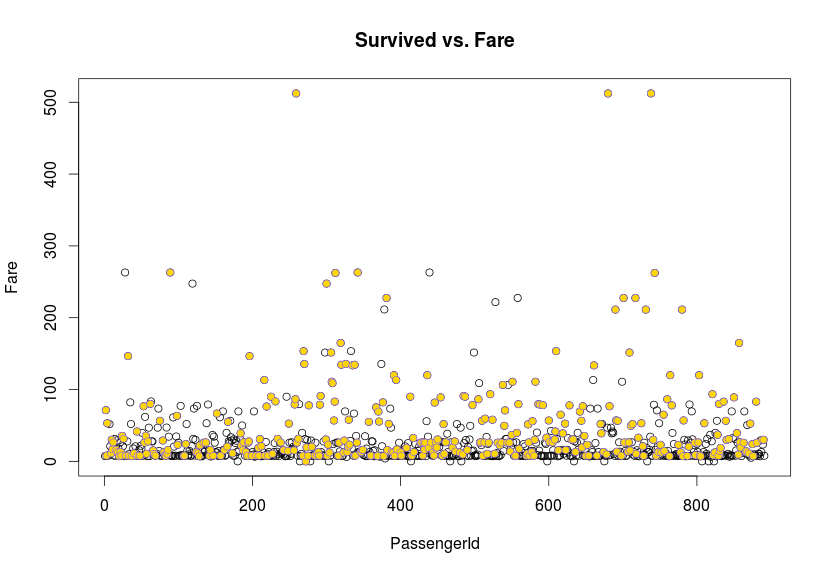
\includegraphics[scale=0.40]{images/survived-vs-fare.png}
\end{center}

15 rekordów ma wartość 0, dlatego potraktowaliśmy je jako braki danych, które uzupełniliśmy medianą dla klasy. Poniższy wykres pokazuje zależność między tymi dwiema zmiennymi.

\begin{center}
	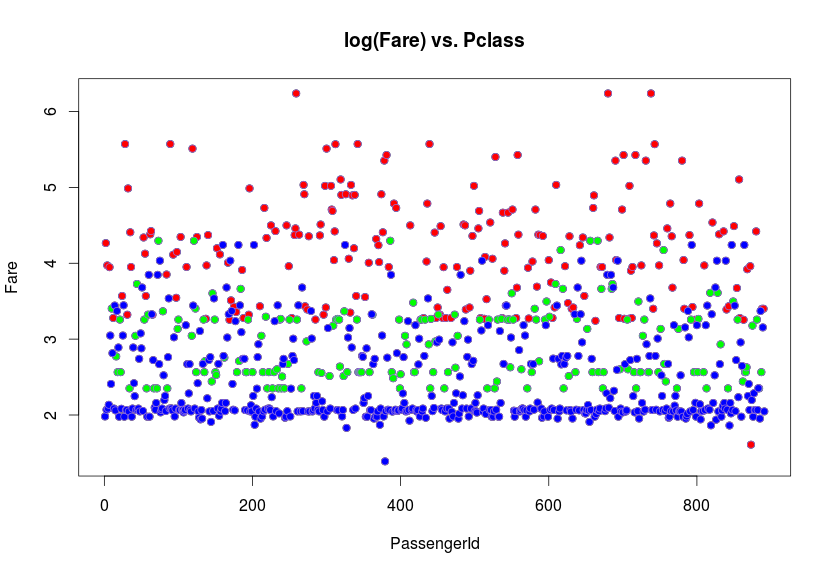
\includegraphics[scale=0.40]{images/logfare-vs-pclass.png}
\end{center}

Widać, że istnieje zależność między klasą a opłatą, w związku z czym 15 braków uzupełniliśmy medianą dla klasy.

\subsection{Miejsce wejścia na pokład }

Większość pasażerów okrętowało się w Southampton, dlatego 2 brakujące rekordy zastąpione tym właśnie portem.
\begin{center}
    \begin{tabular}{| l | l | l | l |}
    \hline
        &  C &  Q &  S  \\ \hline
      2 & 168 & 77 & 644  \\
    \hline
    \end{tabular}
\end{center}

Ku naszemu zaskoczeniu, widać, że wartości tego atrybutu posiadają korelację z wpływem na przeżycie osoby podróżującej.

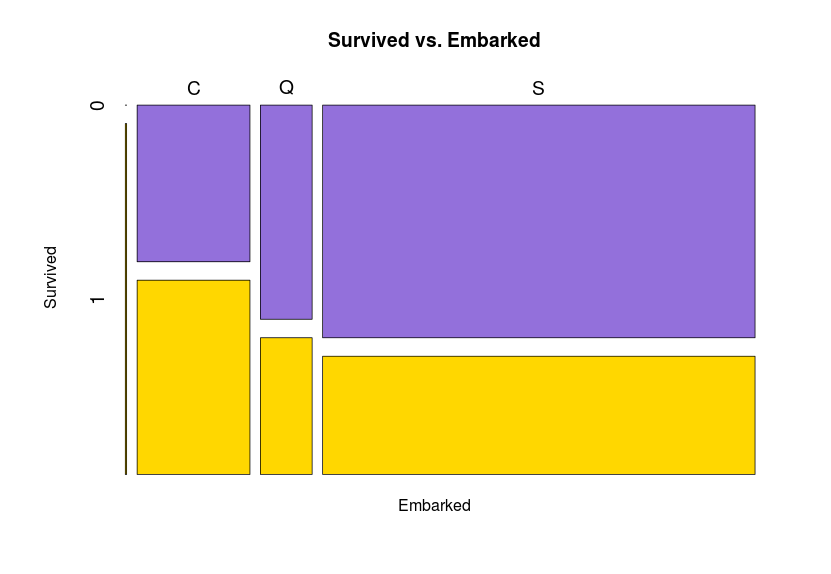
\includegraphics[scale=0.40]{images/survived-vs-embarked.png}

\subsection{Atrybuty, których nie bierzemy pod uwagę}
Część atrybutów ze zbioru danych nie została uwzględniona przez nas w eksperymentów.

\subsubsection{Identyfikator pasażera}
Jest to zmienna porządkowa, identyfikator pasażera w zbiorze danych -- nie ma sensu tego uwzględniać.

\subsubsection{Przeżycie}
Jest to atrybut objaśniany, dlatego nie możemy go użyć do budowy modelu.

\subsubsection{Imię i nazwisko}
Na początku uznaliśmy, że ten atrybut również możemy pominąć, w związku z czym ta kolumna nie jest uwzględniona w eksperymentach.
Potem zauważyliśmy, że poza imieniem i nazwiskiem zawarty jest także tytuł. Naszym pomysłem, którego nei zdążyliśmy zrealizować,
jest podzielenie tej kolumny na 4 klasy: panna, pani, pan (nieżonaty) i pan (żonaty). Taki podział wydaje się sensowniejszy od imienia i nazwiska,
więc prawdopodobnie mogłoby to wpłynąć na budowane modele.

\subsubsection{Numer biletu}
Ten atrybut zawiera wartości alfanumeryczne. Nie udało nam się wymyślić w jaki sposób możemy tego użyc przy analizie.

\subsubsection{Kajuta}
Z racji na 687 braków (w 891 próbkach) uznaliśmy, że tą zmienną pominiemy.
Inną możliwościa jest próba użycia jej do lepszej klasyfikacji osób, które mają wartość dla tej zmiennej, ale tego również nie zrobiliśmy.

\section{Selekcja atrybutów}
\label{attrSelec}
\section{Kalibracja}
\subsection{Drzewo}
Drzewo możemy kalibrować poprzez odcięcie w odpowiednim momencie. Zgodnie z dokumentacją {\itshape rpart} należy to przyciąć dla parametru $cp$
dla pierwszej kropki poniżej linii przerywanej na poniższym wykresie. Oznacza to, że przy generowaniu modelu z użyciem drzewa losowego, parametr $cp$ należy ustawić na $0.01$.

\begin{center}
	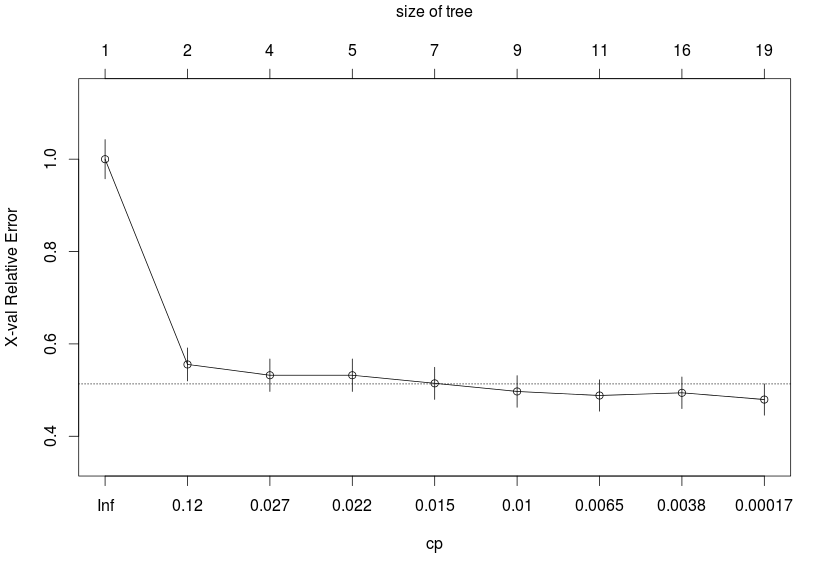
\includegraphics[scale=0.40]{images/przycinanie.png}
\end{center}

\subsection{KNN}
\label{knncalib}
Metodę $K$-najbliższych sąsiadów można parametryzować przez liczbę głosujących sąsiadów. Poniższy wykres przedstawia zależność celności modelu w zależności od liczby sąsiadów.

\begin{center}
	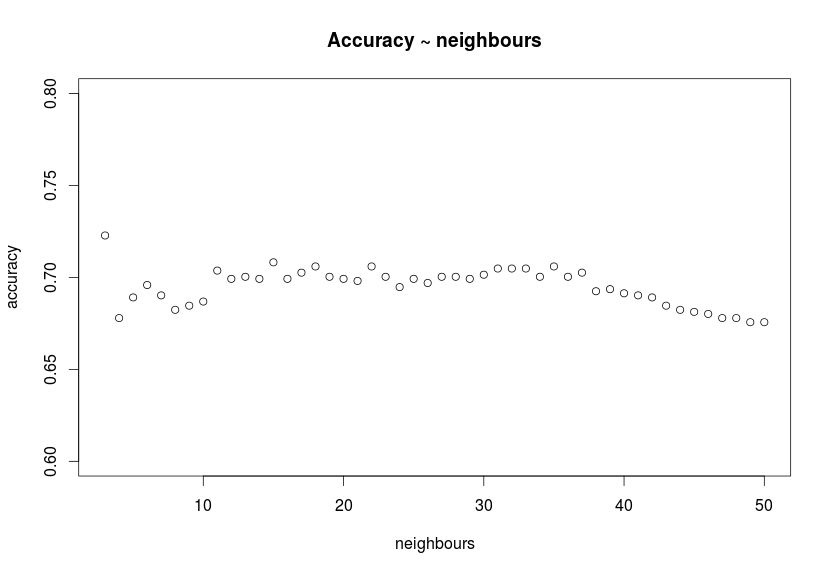
\includegraphics[scale=0.40]{images/accuracy-neighbours50.png}
\end{center}

Jak łatwo zauważyć celnośc na początku jest raczej stabilna, natomiast potem zaczyna spadać liniowo. Najlepszą celność uzyskaliśmy dla liczby sąsiadów $3$, dlatego takiej wartości użyliśmy przy eksperymentach.

\section{Tworzenie modeli}

Dla każdego algorytmu klasyfikacji użyto danych poddanych selekcji przedstawionej w sekcji \ref{attrSelec}. Dodatkowo wykorzystaliśmy algorytm PCA w celu redukcji wymiarowości danych, a następnie sprawdziliśmy jakość modelu po redukcji wymiarowości danych. Do tworzenia modelu i testowania jego jakości wykorzystaliśmy metodę kroswalidacji. W celu wizualnego przedstawienia jakości wytworzonego modelu dla każdego eksperymentu wygenerowana została krzywa ROC. 

\subsection{Naiwny Bayes}

Dla danych po selekcji atrybutów z sekcji \ref{attrSelec}, bez redukcji wymiarowości danych:

\begin{center}
    \begin{tabular}{| l | l | l | l | l|}
    \hline
        Dokładność &  Precyzja &  Czułość & Specyficzność \\ \hline
      	0.7856341 & 0.7253731 & 0.7105263 & 0.8324226  \\
    \hline
    \end{tabular}
\end{center}

\begin{center}
	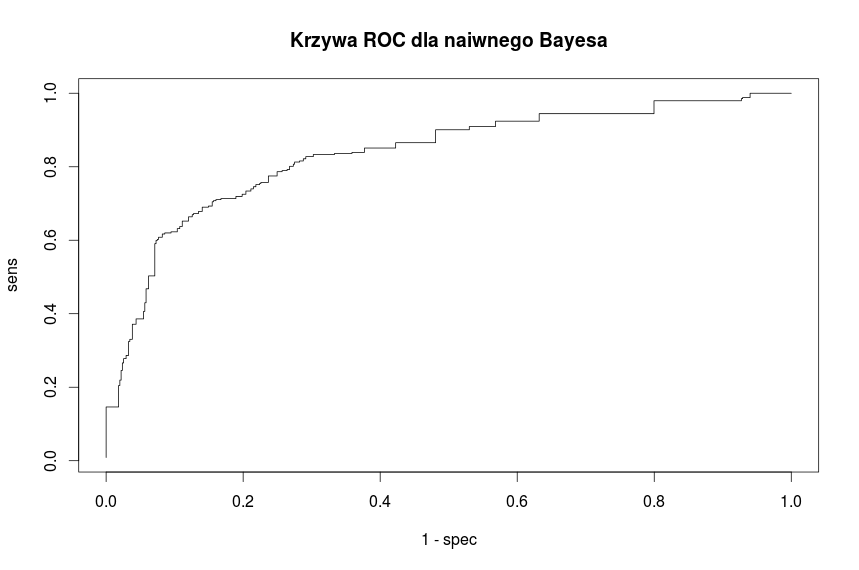
\includegraphics[scale=0.40]{images/bayesNoPCA.png}
\end{center}

Współczynnik AUC (pole powierzchni pod krzywą ROC) wyniosło 0.8341482.

Po przetworzeniu danych przez PCA i redukcji jednego wymiaru:

\begin{center}
    \begin{tabular}{| l | l | l | l | l|}
    \hline
        Dokładność &  Precyzja &  Czułość & Specyficzność \\ \hline
      	0.7890011 & 0.7319277 & 0.7105263 & 0.8378871  \\
    \hline
    \end{tabular}
\end{center}

\begin{center}
	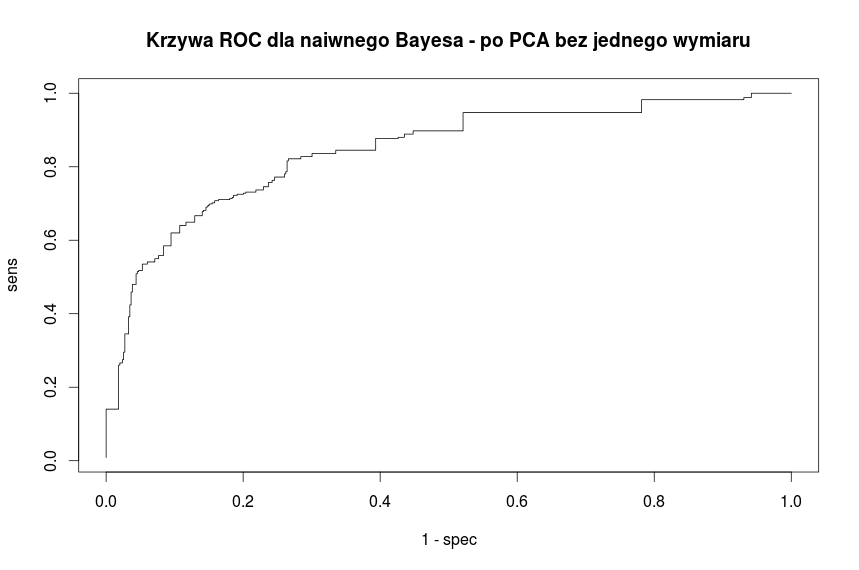
\includegraphics[scale=0.40]{images/bayes1.png}
\end{center}

Współczynnik AUC: 0.8438415

Po przetworzeniu danych przez PCA i redukcji dwóch wymiarów:

\begin{center}
    \begin{tabular}{| l | l | l | l | l|}
    \hline
        Dokładność &  Precyzja &  Czułość & Specyficzność \\ \hline
      	0.7609428 & 0.677686 & 0.7192982 & 0.7868852  \\
    \hline
    \end{tabular}
\end{center}

\begin{center}
	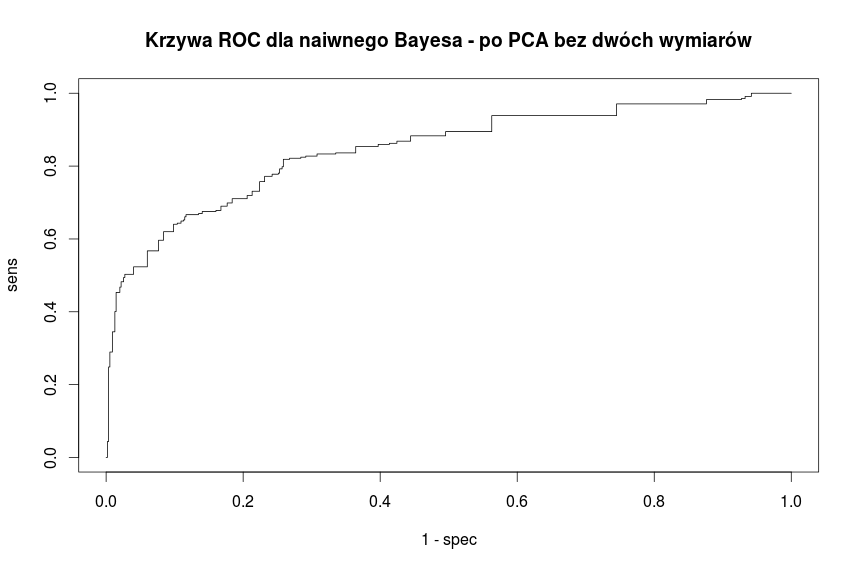
\includegraphics[scale=0.40]{images/bayes2.png}
\end{center}

Współczynnik AUC: 0.8450985

\subsection{Drzewo decyzyjne}

Dla danych po selekcji atrybutów z sekcji \ref{attrSelec}, bez redukcji wymiarowości danych:

\begin{center}
    \begin{tabular}{| l | l | l | l | l|}
    \hline
        Dokładność &  Precyzja &  Czułość & Specyficzność \\ \hline
      	0.8035915 & 0.7889273 & 0.6666667 & 0.8888889 \\
    \hline
    \end{tabular}
\end{center}

\begin{center}
	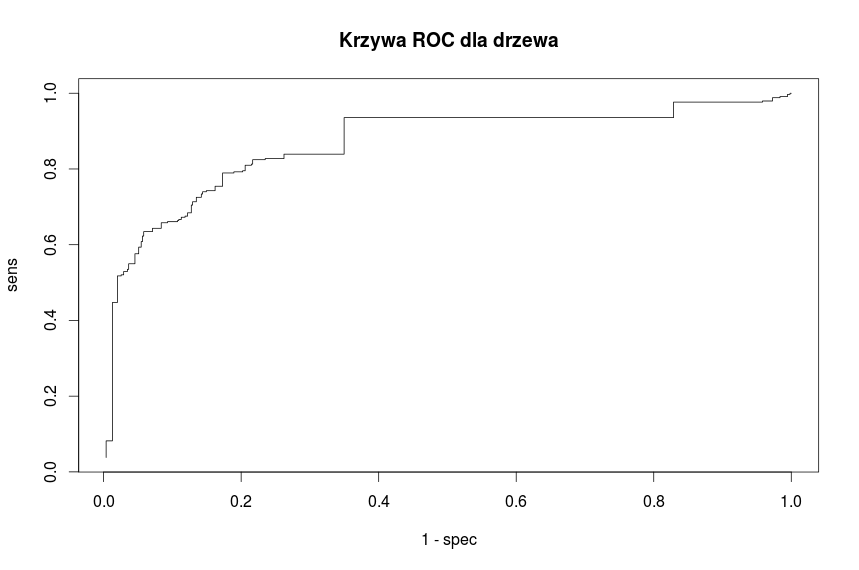
\includegraphics[scale=0.40]{images/treeNoPCA.png}
\end{center}

Współczynnik AUC wyniósł 0.8658379.

Po przetworzeniu danych przez PCA i redukcji jednego wymiaru:

\begin{center}
    \begin{tabular}{| l | l | l | l | l|}
    \hline
        Dokładność &  Precyzja &  Czułość & Specyficzność \\ \hline
      	0.8103255 & 0.7912458 & 0.6871345 & 0.8870674  \\
    \hline
    \end{tabular}
\end{center}

\begin{center}
	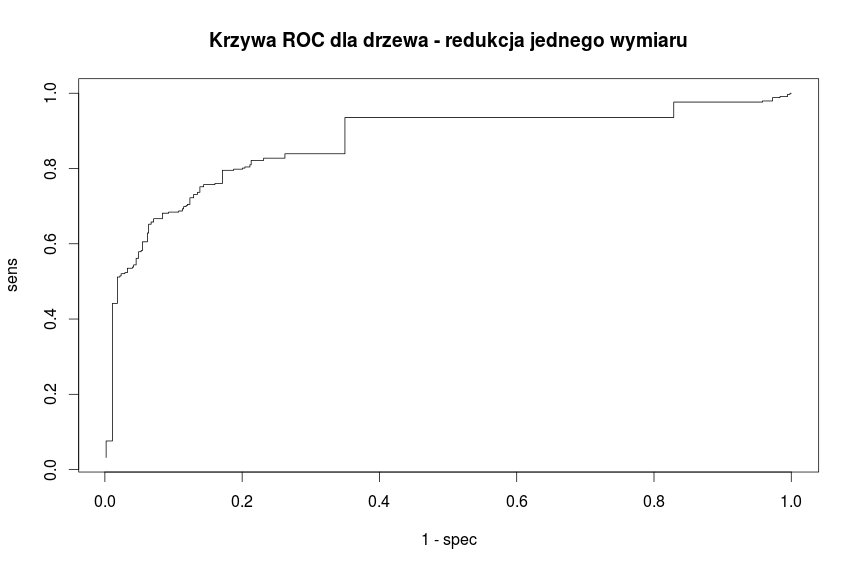
\includegraphics[scale=0.40]{images/tree1.png}
\end{center}

Współczynnik AUC: 0.86873

Po przetworzeniu danych przez PCA i redukcji dwóch wymiarów:

\begin{center}
    \begin{tabular}{| l | l | l | l | l|}
    \hline
        Dokładność &  Precyzja &  Czułość & Specyficzność \\ \hline
      	0.8080808 & 0.7840532 & 0.6900585 & 0.8816029  \\
    \hline
    \end{tabular}
\end{center}

\begin{center}
	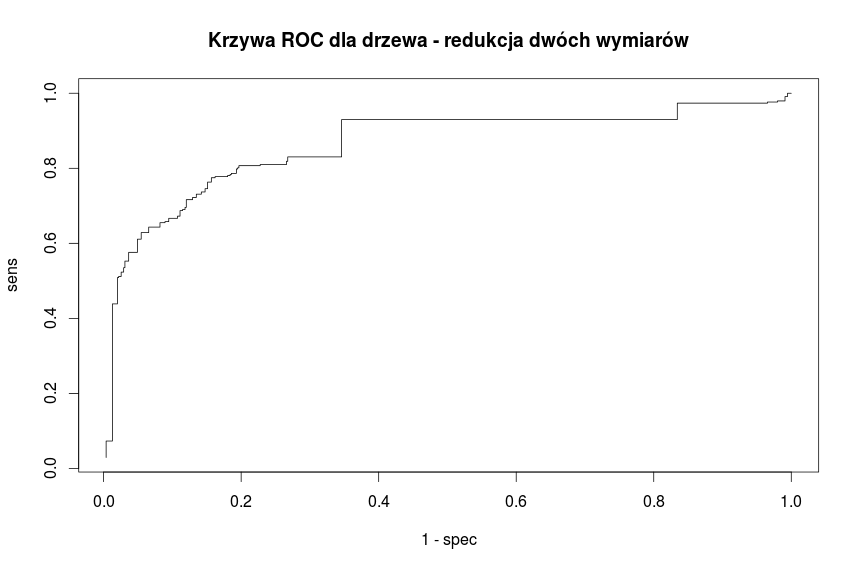
\includegraphics[scale=0.40]{images/tree2.png}
\end{center}

Współczynnik AUC: 0.8623973

Po zmianie parametru $cp=0.015$ i bez redukcji wymiary danych:

\begin{center}
    \begin{tabular}{| l | l | l | l | l|}
    \hline
        Dokładność &  Precyzja &  Czułość & Specyficzność \\ \hline
      	0.8103255 & 0.8078292 & 0.6637427 & 0.9016393 \\
    \hline
    \end{tabular}
\end{center}

\begin{center}
	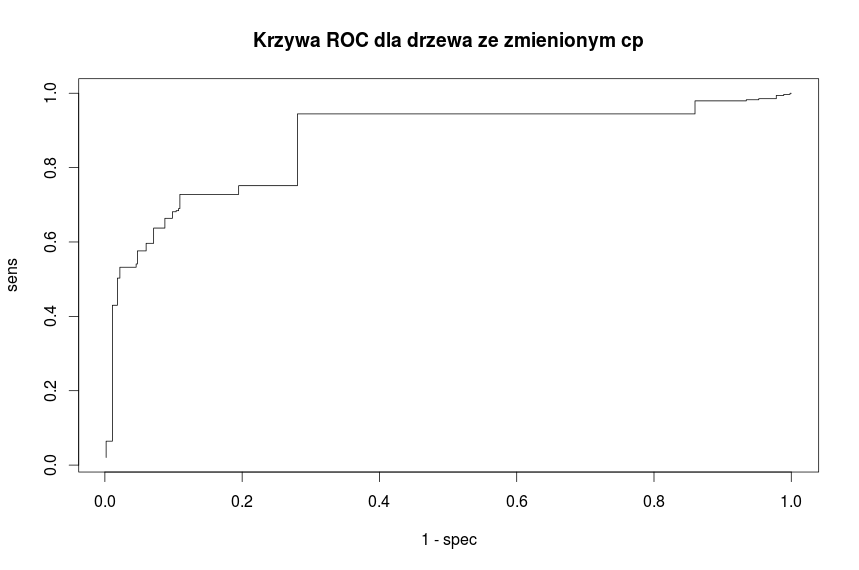
\includegraphics[scale=0.40]{images/cptreeNoPCA.png}
\end{center}

Współczynnik AUC: 0.8698378

Po przetworzeniu danych przez PCA i redukcji jednego wymiaru:

\begin{center}
    \begin{tabular}{| l | l | l | l | l|}
    \hline
        Dokładność &  Precyzja &  Czułość & Specyficzność \\ \hline
      	0.8170595 & 0.8140351 & 0.6783626 & 0.9034608  \\
    \hline
    \end{tabular}
\end{center}

\begin{center}
	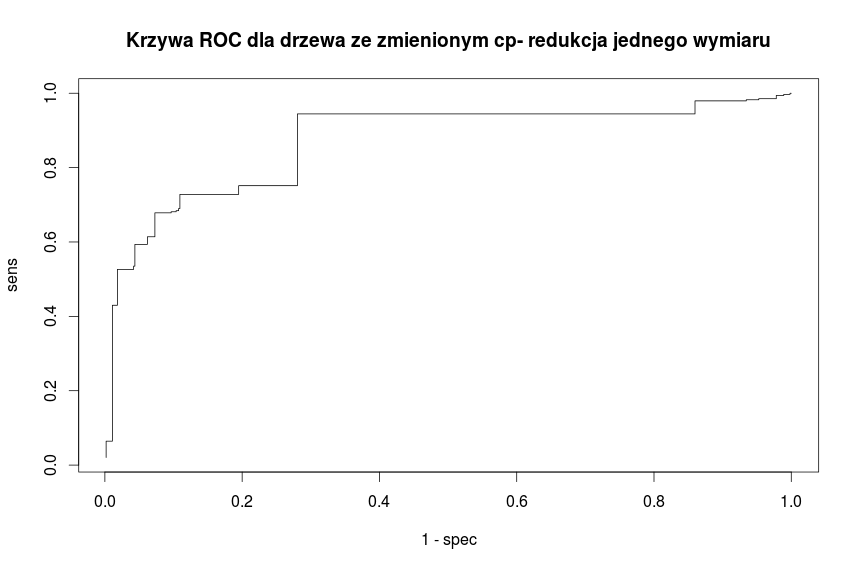
\includegraphics[scale=0.40]{images/cptree1.png}
\end{center}

Współczynnik AUC: 0.871116

Po przetworzeniu danych przez PCA i redukcji dwóch wymiarów:

\begin{center}
    \begin{tabular}{| l | l | l | l | l|}
    \hline
        Dokładność &  Precyzja &  Czułość & Specyficzność \\ \hline
      	0.8125701 & 0.804878 & 0.6754386 & 0.8979964  \\
    \hline
    \end{tabular}
\end{center}

\begin{center}
	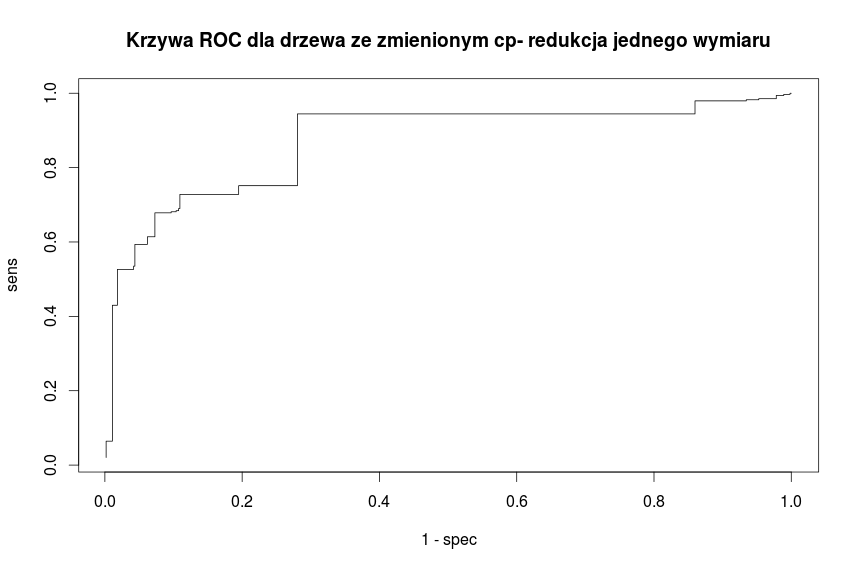
\includegraphics[scale=0.40]{images/cptree2.png}
\end{center}

Współczynnik AUC: 0.8617103.

\subsection{LDA}

Dla danych po selekcji atrybutów z sekcji \ref{attrSelec}, bez redukcji wymiarowości danych:

\begin{center}
    \begin{tabular}{| l | l | l | l | l|}
    \hline
        Dokładność &  Precyzja &  Czułość & Specyficzność \\ \hline
      	0.7934905 & 0.7484277 & 0.6959064 & 0.8542805 \\
    \hline
    \end{tabular}
\end{center}

\begin{center}
	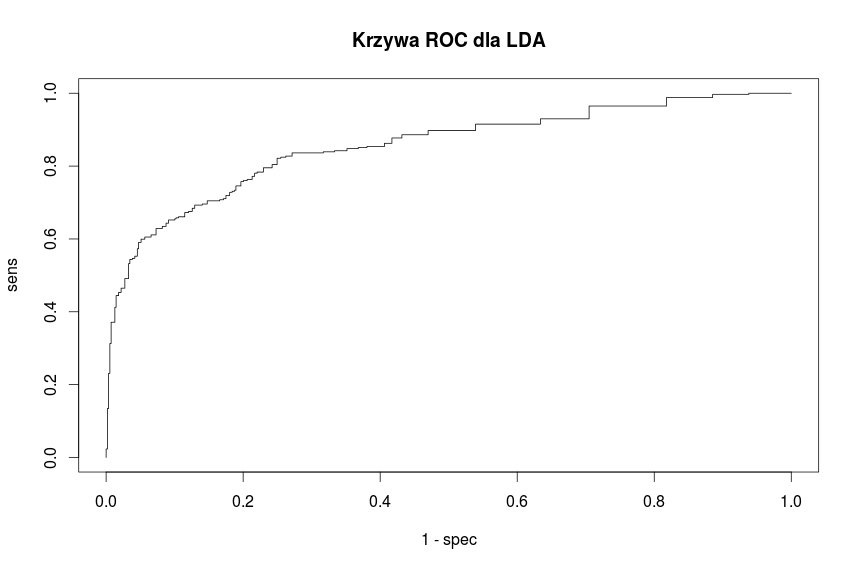
\includegraphics[scale=0.40]{images/ldaNoPCA.png}
\end{center}

Współczynnik AUC wyniósł 0.8549835.

Po przetworzeniu danych przez PCA i redukcji jednego wymiaru:

\begin{center}
    \begin{tabular}{| l | l | l | l | l|}
    \hline
        Dokładność &  Precyzja &  Czułość & Specyficzność \\ \hline
      	0.7890011 & 0.7483871 & 0.6783626 & 0.8579235  \\
    \hline
    \end{tabular}
\end{center}

\begin{center}
	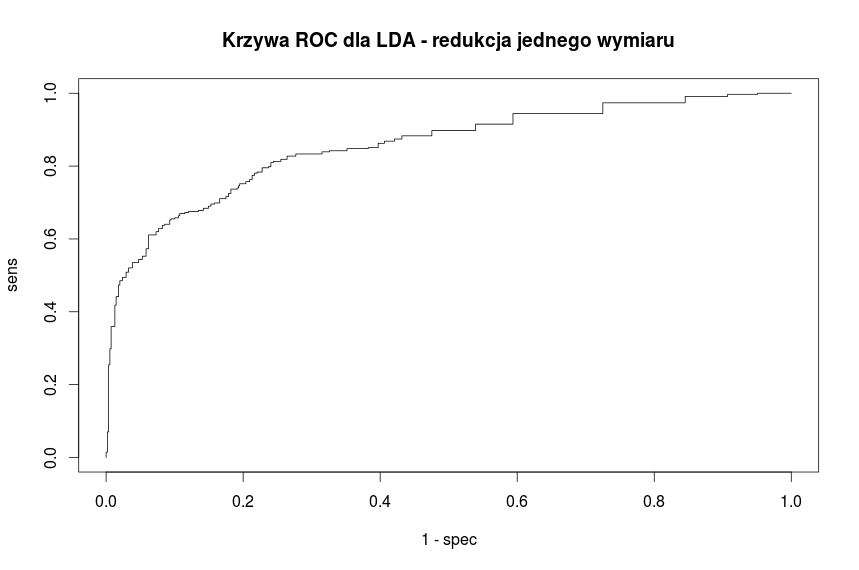
\includegraphics[scale=0.40]{images/lda1.png}
\end{center}

Współczynnik AUC: 0.8555694.

Po przetworzeniu danych przez PCA i redukcji dwóch wymiarów:

\begin{center}
    \begin{tabular}{| l | l | l | l | l|}
    \hline
        Dokładność &  Precyzja &  Czułość & Specyficzność \\ \hline
      	0.7912458 & 0.7532468 & 0.6783626 & 0.8615665  \\
    \hline
    \end{tabular}
\end{center}

\begin{center}
	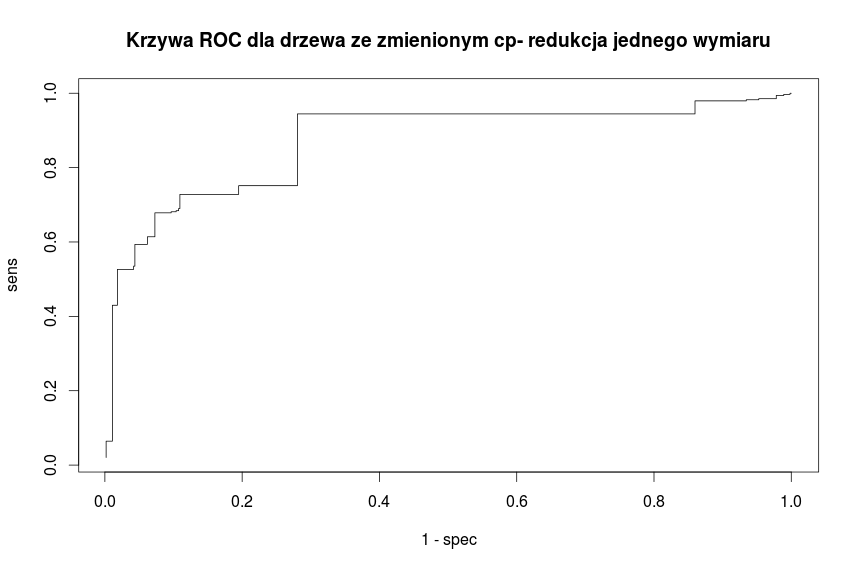
\includegraphics[scale=0.40]{images/cptree2.png}
\end{center}

Współczynnik AUC: 0.8548451.

\subsection{KNN}

Dla KNN obliczone zostały tylko wartości wskaźników. Bazując na przeprowadzonej kalibracji, która została przedstawiona w podrozdziale \ref{knncalib} liczba sąsiadów została ustalona na 20.\\

\begin{center}
    \begin{tabular}{| l | l | l | l | l|}
    \hline
        Dokładność &  Precyzja &  Czułość & Specyficzność \\ \hline
      	0.7070707 & 0.6483516 & 0.5175439 & 0.8251366  \\
    \hline
    \end{tabular}
\end{center}

\section{Ocena jakości modeli}
\section{Podsumowanie}
Podczas projektu analizowaliśmy dane dotyczące pasażerów Titanica. Udało nam się stworzyć modele obrazujące zależność między pewnymi atrybutami pasażera, a szansą przeżycia.

Przed wykonaniem modeli dokonaliśmy analizy danych pod kątem możliwości użycia w budowanych modelach. Części danych nie udało nam się wykorzystać.
W częsci musieliśmy uzupełnić braki. Przyjęliśmy, że lepiej będziemy mogli porównać modele używając w każdym z nich dokładnie tych samych danych,
niezależnie od tego czy metoda radzi sobie z brakami, czy nie.

Następnie użyliśmy algorytmu PCA, aby usunąć najmniej istotne kolumny. Pozwoliło to zbadać wpływ użytych kolumn na uzyskane wyniki.

Część modeli wykalibrowaliśmy: drzewo ucięliśmy, natomiast w metodzie KNN zbadaliśmy wpływ liczby sąsiadów.

Uzyskane modele porównaliśmy pod kątem pola pod krzywą ROC oraz parametrów czułości, specyficzności, precyzji i dokładności.
Wszystkie modele (dla których można narysować krzywą ROC) miały "wypukłą" krzywą, ponad linią prostej losowej.

Projekt pozwolił nam lepiej zrozumieć proces analizowania i klasyfikacji danych.

\end{document}
